
\documentclass[compress]{beamer}
\usepackage{ifthen,verbatim}

\newcommand{\isnote}{}
\xdefinecolor{lightyellow}{rgb}{1.,1.,0.25}
\xdefinecolor{darkblue}{rgb}{0.1,0.1,0.7}

%% Uncomment this to get annotations
%% \def\notes{\addtocounter{page}{-1}
%%            \renewcommand{\isnote}{*}
%% 	   \beamertemplateshadingbackground{lightyellow}{white}
%%            \begin{frame}
%%            \frametitle{Notes for the previous page (page \insertpagenumber)}
%%            \itemize}
%% \def\endnotes{\enditemize
%% 	      \end{frame}
%%               \beamertemplateshadingbackground{white}{white}
%%               \renewcommand{\isnote}{}}

%% Uncomment this to not get annotations
\def\notes{\comment}
\def\endnotes{\endcomment}

\setbeamertemplate{navigation symbols}{}
\setbeamertemplate{headline}{\mbox{ } \hfill
\begin{minipage}{5.5 cm}
\vspace{-0.75 cm} \small
\end{minipage} \hfill
\begin{minipage}{4.5 cm}
\vspace{-0.75 cm} \small
\begin{flushright}
\ifthenelse{\equal{\insertpagenumber}{1}}{}{\hspace{0.2 cm} \insertpagenumber\isnote/\pageref{numpages}}
\end{flushright}
\end{minipage}\mbox{\hspace{0.2 cm}}\includegraphics[height=1 cm]{../cmslogo} \hspace{0.01 cm} \vspace{-1.05 cm}}

\begin{document}
%% \begin{frame}
%% \vfill
%% \begin{center}
%% \textcolor{darkblue}{\Large }

%% \vfill
%% \begin{columns}
%% \column{0.3\linewidth}
%% \begin{center}
%% \large
%% \textcolor{darkblue}{Jim Pivarski}
%% \end{center}
%% \end{columns}

%% \begin{columns}
%% \column{0.3\linewidth}
%% \begin{center}
%% \scriptsize
%% {\it Texas A\&M University}
%% \end{center}
%% \end{columns}

%% \vfill
%% 28 October, 2008

%% \end{center}
%% \end{frame}

%% \begin{notes}
%% \item This is the annotated version of my talk.
%% \item If you want the version that I am presenting, download the one
%% labeled ``slides'' on Indico (or just ignore these yellow pages).
%% \item The annotated version is provided for extra detail and a written
%% record of comments that I intend to make orally.
%% \item Yellow notes refer to the content on the {\it previous} page.
%% \item All other slides are identical for the two versions.
%% \end{notes}

\small

\begin{frame}
\frametitle{Early trigger conditions}
\begin{itemize}\setlength{\itemsep}{0.2 cm}
\item Prescales, definitions, and even names in trigger menu may
  change rapidly in response to unknowns in early collisions
\item AlCaReco is bound to a release cycle, can't update as quickly
\item \textcolor{blue}{Old idea:} take an ``OR'' of all available
  triggers of one type \\ (e.g.\ inclusive muon), at least one will
  collect data
\item \textcolor{blue}{Problem:} unable to take advantage of new trigger name
\item \textcolor{blue}{Sub-problem:} current code throws exceptions
  when it encounters an unknown name; we're getting a parameter to
  turn that off
\end{itemize}

\vspace{0.2 cm}
\hspace{-0.83 cm} \textcolor{darkblue}{\Large Conclusions from HLT/AlCaReco meeting}

\vspace{0.05 cm}
\begin{enumerate}
\item Disappearing/changing trigger names would only happen in emergencies, with a reversion time of $\sim$24 hours
\item We could move our trigger selection to the offline database
\end{enumerate}
\end{frame}

\begin{frame}
\frametitle{Trigger selection in offline database}

\textcolor{darkblue}{Current method}

\vspace{0.2 cm}
\includegraphics[width=\linewidth]{before_database.png}

\vfill
\textcolor{darkblue}{Access via database}

\vspace{0.2 cm}
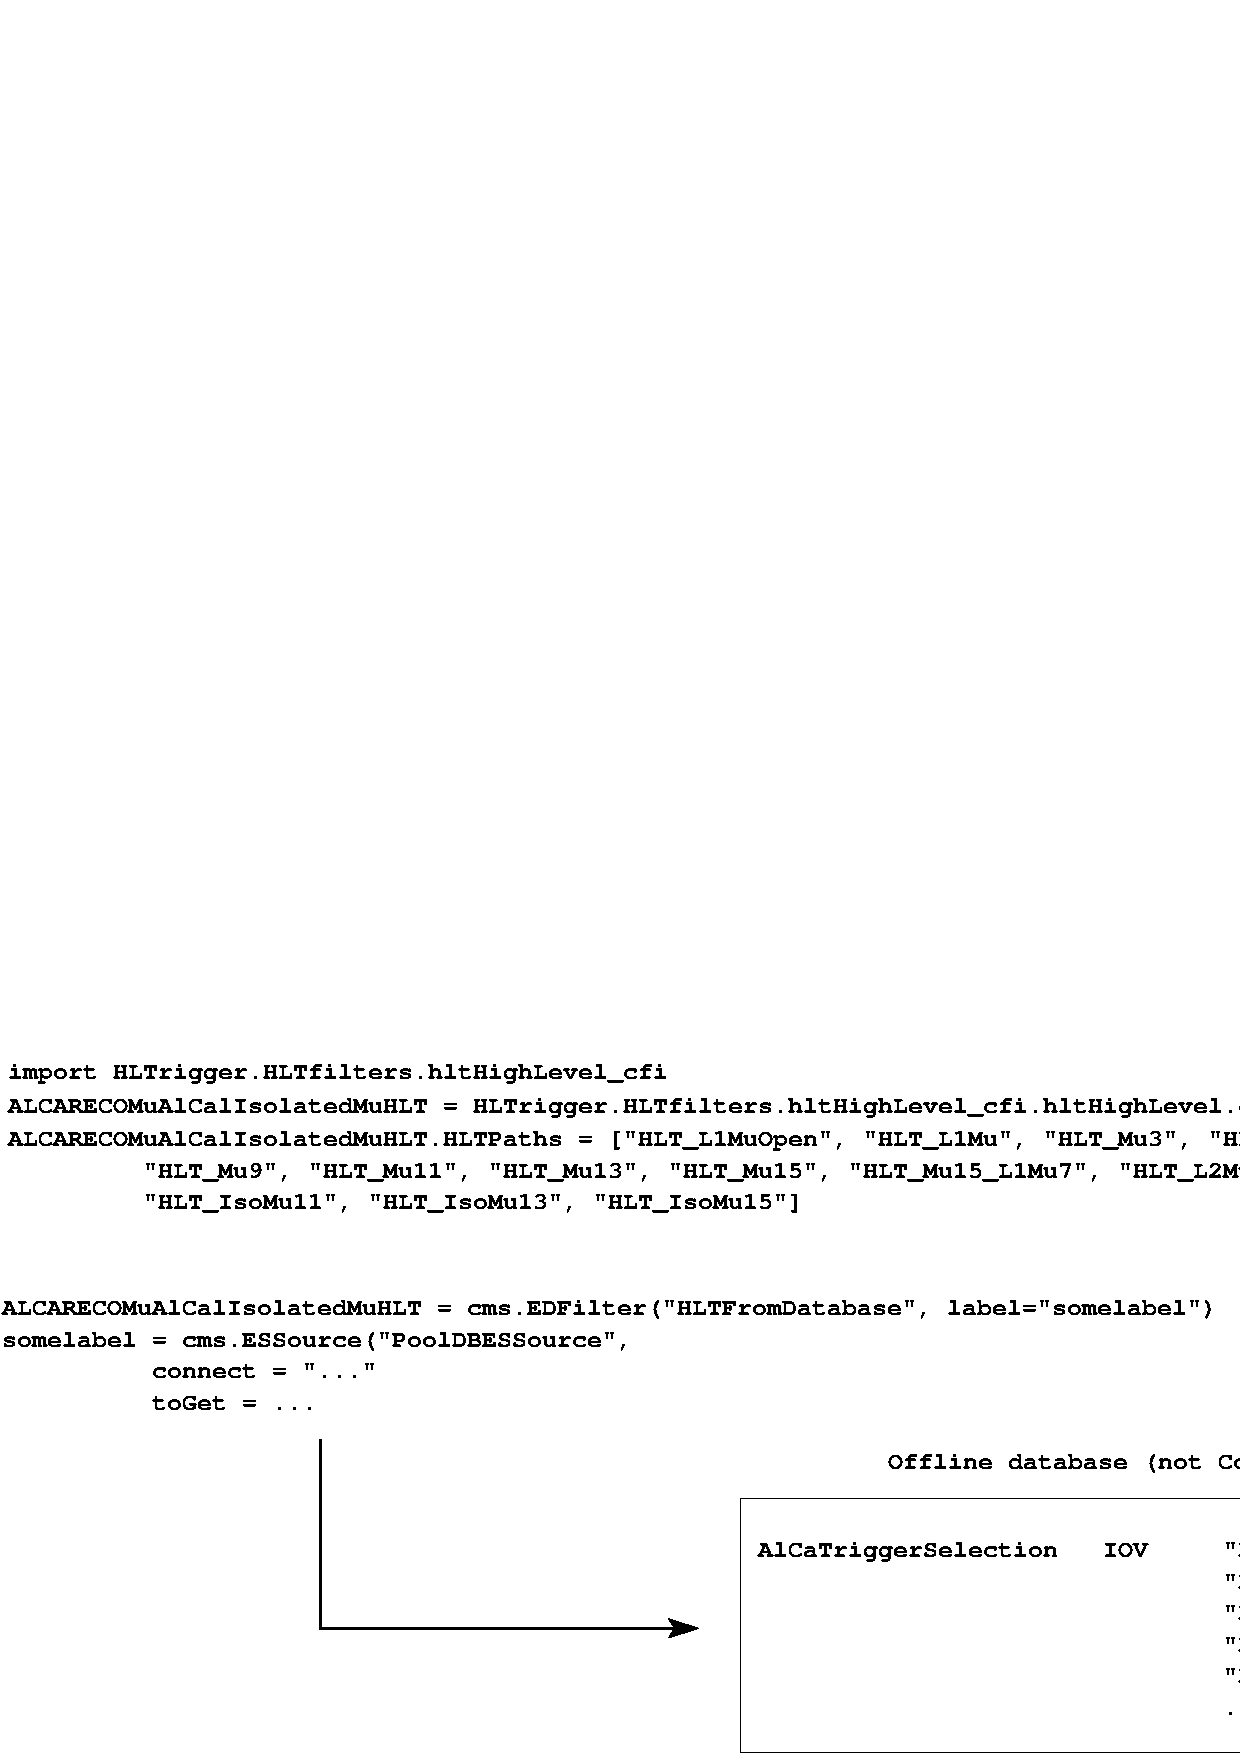
\includegraphics[width=\linewidth]{database.png}

\vfill
\begin{itemize}
\item Associates trigger selection with run number (IOV) to better match trigger scenario during data-taking

\item In the very early stages of development
\end{itemize}
\end{frame}

\begin{frame}
\frametitle{Do all AlCaRecos need to select trigger names?}

\vfill
\begin{itemize}\setlength{\itemsep}{0.5 cm}

\item Of course trigger definitions affect all data collection,
  including AlCaRecos, but some AlCaReco configurations don't need to
  explicitly select a set of names

\item Explicit AlCaReco trigger name selection not relevant for rate
  because it happens after reconstruction

\vspace{0.1 cm}

\includegraphics[width=\linewidth]{alca_path2.png}

\item AlCaRecos must be associated with relevant primary datasets: \\ in
  some cases, this provides all the filtering an explicit trigger name
  requirement would have (e.g.\ cosmic rays, beam-halo)

\item This simplification would reduce the amount of work we need to
  do to keep up with changes in the trigger, without loss in many cases

\end{itemize}

\end{frame}


\begin{frame}
\frametitle{Example: Muon Alignment AlCaRecos}
\scriptsize
\renewcommand{\arraystretch}{1.3}

\vfill
\begin{tabular}{p{0.1 cm} p{0.3\linewidth} p{0.3\linewidth} p{0.3\linewidth}}
& Muon AlCaReco Stream & trigger & Comments \\\hline
E & MuAlCalIsolatedMu & none & muon $p_T$ cut is higher than HLT \\
E? & MuAlOverlaps & none & track pattern recognition is a tighter cut than HLT \\
P & MuAlZMuMu & none & dimuon mass cut is tighter than HLT \\
P & MuAlStandAloneCosmics & cosmic ray tech.\ trigger & special primary dataset for special reco path \\  %  (``24 OR 25 OR 26 OR 27 OR 28'')
P & MuAlGlobalCosmics & same as above & \\
P & MuAlBeamHalo & L1\_SingleMuBeamHalo/ HLT\_CSCBeamHalo & may or may not be \mbox{separate} from cosmics \\
P & MuAlBeamHaloOverlaps & same as above & \\
\end{tabular}

\vfill
\begin{itemize}\setlength{\itemsep}{0.2 cm}
\item ``E'' labels Express Streams (no Primary Datasets), ``P'' labels Prompt Reconstruction (split into Primary Datasets)
\item ``none'' means no explicit selection, though event distribution is determined by union of all active triggers, selected afterward for muons
\end{itemize}

%% \hspace{-0.83 cm} \textcolor{darkblue}{\Large Outline2}
\label{numpages}
\end{frame}

%% \begin{frame}
%% \frametitle{Some context}

%% \begin{itemize}
%% \item Only Prompt Reco can have non-standard reconstruction paths

%% \mbox{ } \hfill \includegraphics[width=0.6\linewidth]{alcareco_path.png} \hfill \mbox{ }

%% \item HLT selection is not a question of algorithmic speed, \mbox{but backgrounds\hspace{-1 cm}}

%% \mbox{ } \hfill 
\includegraphics[width=0.8\linewidth]{alca_path2.png} \hfill \mbox{ }

%% \item Do HLT filters reject more backgrounds than the AlCa
%%   object-based selection?  Could that processing be replicated in the
%%   AlCa step?

%% \end{itemize}
%% \end{frame}

%% \section*{First section}
%% \begin{frame}
%% \begin{center}
%% \Huge \textcolor{blue}{First section}
%% \end{center}
%% \end{frame}

%% \begin{frame}
%% \label{numpages}
%% \end{frame}

\end{document}
